\documentclass{article}

\usepackage{ctex}
\usepackage{listings}
\usepackage[framed,numbered,autolinebreaks,useliterate]{mcode}
\usepackage{geometry}
\usepackage{graphicx}
\usepackage{float}
\geometry{a4paper, scale=0.8}

\title{数学实验实验报告}
\author{ZhaohengLi 2017050025\\cainetatum@foxmail.com\\15801206130}

\begin{document}
\maketitle
\section{实验目的}
\begin{itemize}
	\item{掌握用MATLAB软件求微分方程初值问题数值解的方法;}
	\item{通过实例学习用微分方程模型解决简化的实际问题;}
	\item{了解欧拉方法和龙格—库塔方法的基本思想和计算公式,及稳定性等概念;}
	\item{练习数值微分的计算。}
\end{itemize}

\newpage
\section{CH4-T5 放射性废物处理}

\subsection{建立模型}
通过对海中正在下降的圆筒作受力分析,可以发现圆筒受重力 G,浮力 F 和阻力 f 的 影响,设圆筒质量为 m,重力加速度为 g,则 G = mg,阻力与下沉速度比例系数为$\alpha$。当 桶的下降速度为 v 时,列出受力方程如下:
$$\frac{dv}{dt}=\frac{G-F-\alpha v}{m}$$
对于初值,假设桶从速度为0开始自由下落,即$v(0)=0$。

\subsection{解析解法}
对于上述一阶非齐次线性微分方程,直接代入通解公式即可得到:
$$v=\frac{G-F}{\alpha}(1-e^{-\frac{\alpha}{m}t})$$
此时,桶已经下降的深度为(假设 h(0) = 0):
$$h=\int^{t}_{0}v(\tau)d\tau=\frac{G-F}{\alpha}(t+\frac{m}{a}e^{-\frac{\alpha}{m}t})-\frac{m(G-F)}{\alpha^2}$$
首先,代入题中所给的数据,根据上面导出的 v(t) 解析式反解出当 v = 40ft/s 时的时间。得到 t = 11.8243s。再将这个数值代入 h(t) 中求解下落深度,得到 h = 238.76ft。可以 看出,当速度已经达到 40ft/s 时,桶还没有到达海底,因此桶会发生破裂。此外,也可以画 出桶的下降速度和下落深度随时间的变化图像。从图像中可以明显地看出,当 深度未达到 300 英尺时,速度已经超过 40 英尺每秒。因此桶会与海底冲撞而发生破裂,工 程师赢得了官司。
\begin{figure}[H]
    \centering
    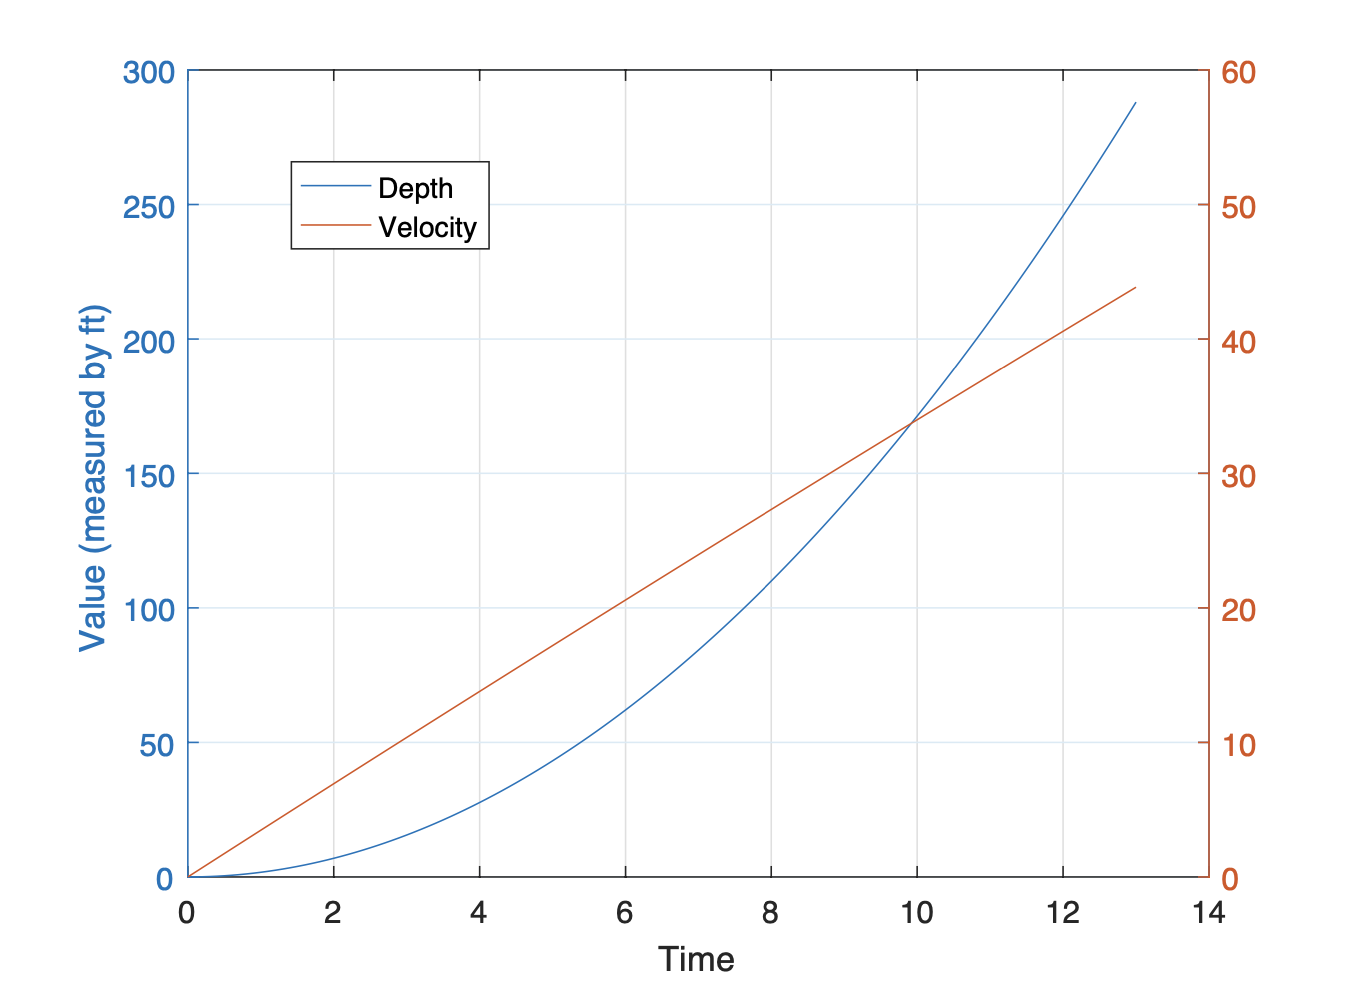
\includegraphics[width=0.7\textwidth]{pic7.png}
    \caption{桶的下降速度和下落深度随时间的变化图像 -解析解法}
\end{figure}

\subsection{数值解法}
根据模型可知,该微分方程可以使用龙格-库塔方法进行数值求解,且满足指定 的精度需求。因此使用 MATLAB 中自带的 ode45 公式进行数值求解,并根据情况 调整计算精度。此外,为了计算桶的下落高度,需要进行积分操作,这里使用的是上一个实 验所学的trap函数进行计算。

MATLAB程序如下:
\begin{lstlisting}
%% Global variables
global m;
global G;
global F;
global alpha;
m = 527.436 * 0.4536;
g = 9.8;
G = m * g;
F = 470.327 * 0.4536 * 9.8;
alpha = 0.08 * 0.4536 * 9.8 / 0.3048;
depth_water = 300 * 0.3048;
speed_limit = 40 * 0.3048;
%% Runge Kutta Method for velocity estimation
ts = 0:0.1:13;
v0 = 0;
[t, v] = ode45(@vpartial, ts, v0);
%% Linear integral for depth integral
h = [0];
for i = 2:length(t)
h = [h; trapz(t(1:i), v(1:i))];
end
%% Plot the figure
[AX] = plotyy(t,h / 0.3048,t,v / 0.3048); grid on;
set(AX(1), 'yTick', 0:50:300);
set(AX(2), 'yTick', 0:10:60);
xlabel('Time');
ylabel('Value (measured by ft)');
legend('Depth', 'Velocity');

%% Fuction
function [ dx ] = vpartial( t, x )
% Global variables
global m;
global G;
global F;
global alpha;
% RHS of the equation
dx = (G - F - alpha * x) / m;
end
\end{lstlisting}


\subsection{计算结果}

程序执行之后,深度与速度随时间的变化如表中数据所示。画出的图像如图所示。 可以看出,使用数值解法与解析解法所得到的图像基本相同。约 11.9 秒时,桶的下落速
度达到 40ft/s,而此时下落高度约 240ft,没有到达海底,速度有效。

\textbf{结论} 桶会与海底冲撞而发生破裂,工程师赢得了官司。

\begin{figure}[H]
    \centering
    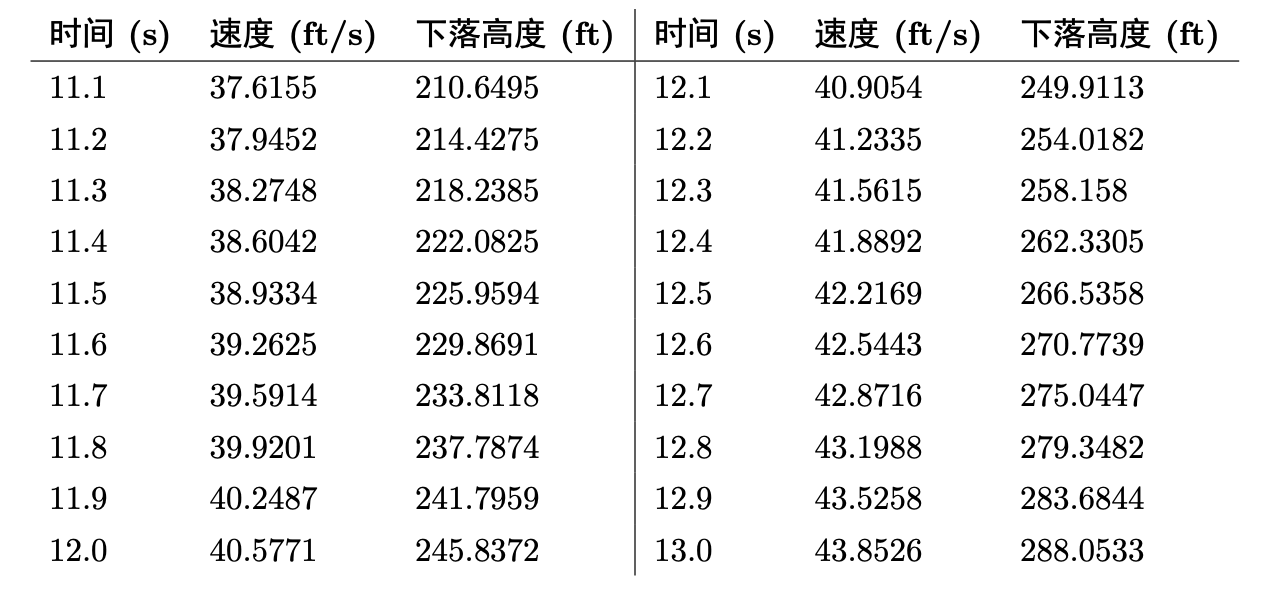
\includegraphics[width=0.7\textwidth]{table61.png}
    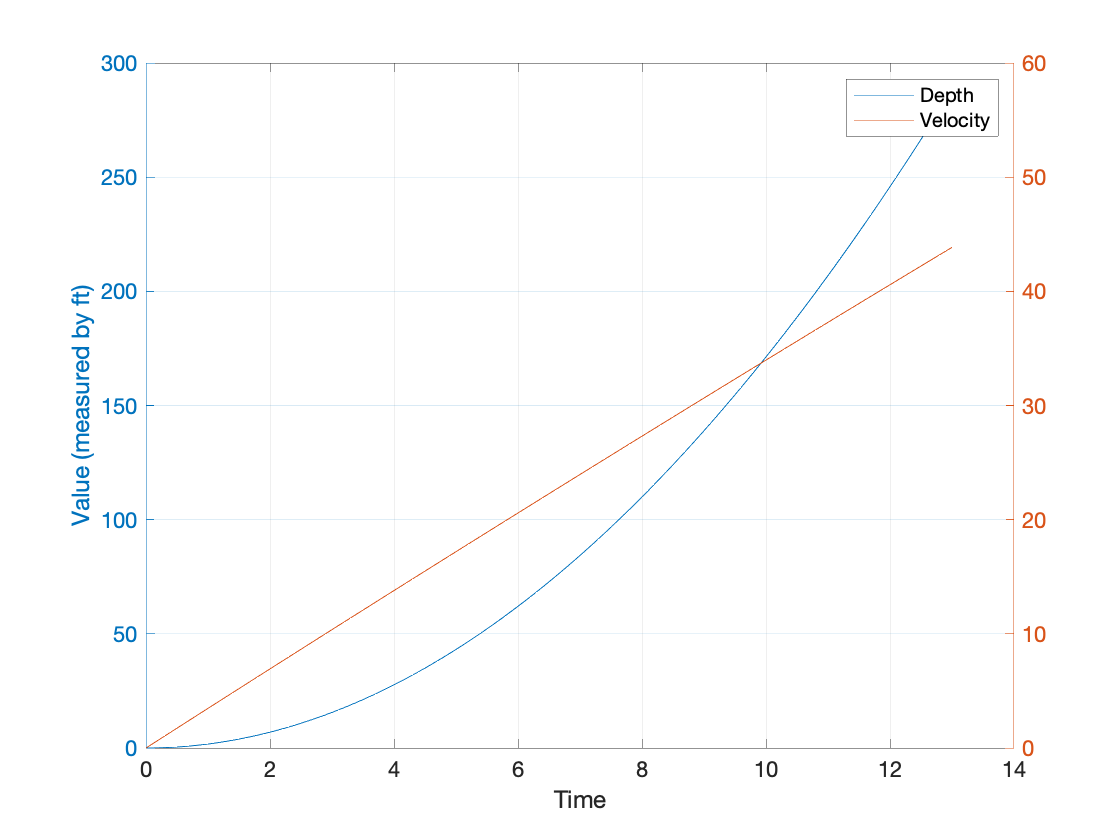
\includegraphics[width=0.7\textwidth]{pic8.png}
    \caption{桶的下降速度和下落深度随时间的变化图像-数值解法}
\end{figure}


\newpage

\section{CH4-T6 小船渡河}
\subsection{建立描述小船航线的数学模型,求其解析解;}
首先建立平面直角坐标系,以 B 点为原点,正右方(即河水流动方向)为 x 轴正方向, 正下方为 y 轴方向。在此坐标系下,A 点坐标为 (0, d),B 点坐标为 (0, 0),设小船坐标为 (x, y)。

将小船的航行速度 v 分解为河水流速 v1 和静水速度 v2,并设向量 (x, y) 与 x 轴夹角为 θ。则有下式成立:
$$\frac{dx}{dt}=v_1-v_2cos\theta$$
$$\frac{dy}{dt}=-v_2sin\theta$$
消除dt得到:
$$\frac{dx}{dy}=\frac{k-cos\theta}{-sin\theta}$$
由$sin\theta=\frac{y}{\sqrt{x^2+y^2}}$和$cos\theta=\frac{x}{\sqrt{x^2+y^2}}$并设$p=frac{x}{y}$,则有:
$$\frac{dx}{dy}=\frac{k-\frac{p}{\sqrt{1+p^2}}}{-\sqrt{1+p^2}}=p-k\sqrt{1+p^2}$$
$$\frac{dp}{dy}=\frac{\frac{dx}{dy}y-x}{y^2}=\frac{\frac{dx}{dy}-p}{y}$$
带入化简可得到:
$$y\frac{dp}{dy}+p=p-k\sqrt{1+p^2}$$
上述微分方程可以进行分离变量y和p进行求解:
$$-k\frac{dy}{y}=\frac{dp}{\sqrt{1+p^2}}$$
在两边同时积分:{}
$$-kln(Cy)=ln(p+\sqrt{p^2+1})$$
为了求出 p 和 y 的关系,上式两边同时求指数之后再正负相加,能导出 $\sqrt{1 + p^2}$,p 和
y 的关系。最终化简结果为:
$$p=\frac{x}{y}=\frac{(Cy)^{-k}-(Cy)^k}{2}$$
代入初值 (p = 0, y = d),能够解出 C = d/1 ,因此,小船航线的解析表达式为:
$$x=\frac{y}{2}[(\frac{y}{d})^{-k}-(\frac{y}{d})^k],\quad 0<y\leq d$$
当y=0时,小船到达了终点,这时有:
$$x=\lim\limits_{y\to 0}\frac{1}{2}[(\frac{1}{d})^{-k}y^{-k+1}-(\frac{1}{d})^ky^{k+1}]$$
显然,当 k > 1 时,上式括号内的第一项在 y 趋于 0 时发散,最终小船的航线始终无法到
达 (0, 0) 点,反而会越飘越远。这也和实际情况相符:如果小船的速度不及静水的流速,那 么无论航行多长时间,都无法到达终点。当 k = 1 时,x 最终收敛结果为 $d/2 \neq 0$,此时小船 能够到达岸边,但是终点在 ( d/2 , 0)。而当 k < 1 时,上式收敛,此时 x = 0,即小船能够到达终点。

MATLAB 代码及结果如下:
\begin{lstlisting}
%% Analytical Solutions

% plot
figure;
subplot(1,3,1);
k=0.5;
x_ana = 0:0.1:d;
y_ana = (x_ana./2) .* ((x_ana./d).^(-k) - (x_ana./d).^k);
plot(y_ana,x_ana);
set(gca,'YDir','reverse')
title("k=0.5")

subplot(1,3,2);
k=1;
x_ana = 0:0.1:d;
y_ana = (x_ana./2) .* ((x_ana./d).^(-k) - (x_ana./d).^k);
plot(y_ana,x_ana);
set(gca,'YDir','reverse')
title("k=1")

subplot(1,3,3);
k=1.5;
x_ana = 0:0.1:d;
y_ana = (x_ana./2) .* ((x_ana./d).^(-k) - (x_ana./d).^k);
plot(y_ana,x_ana);
set(gca,'YDir','reverse')
title("k=1.5")

\end{lstlisting}

\begin{figure}[H]
    \centering
    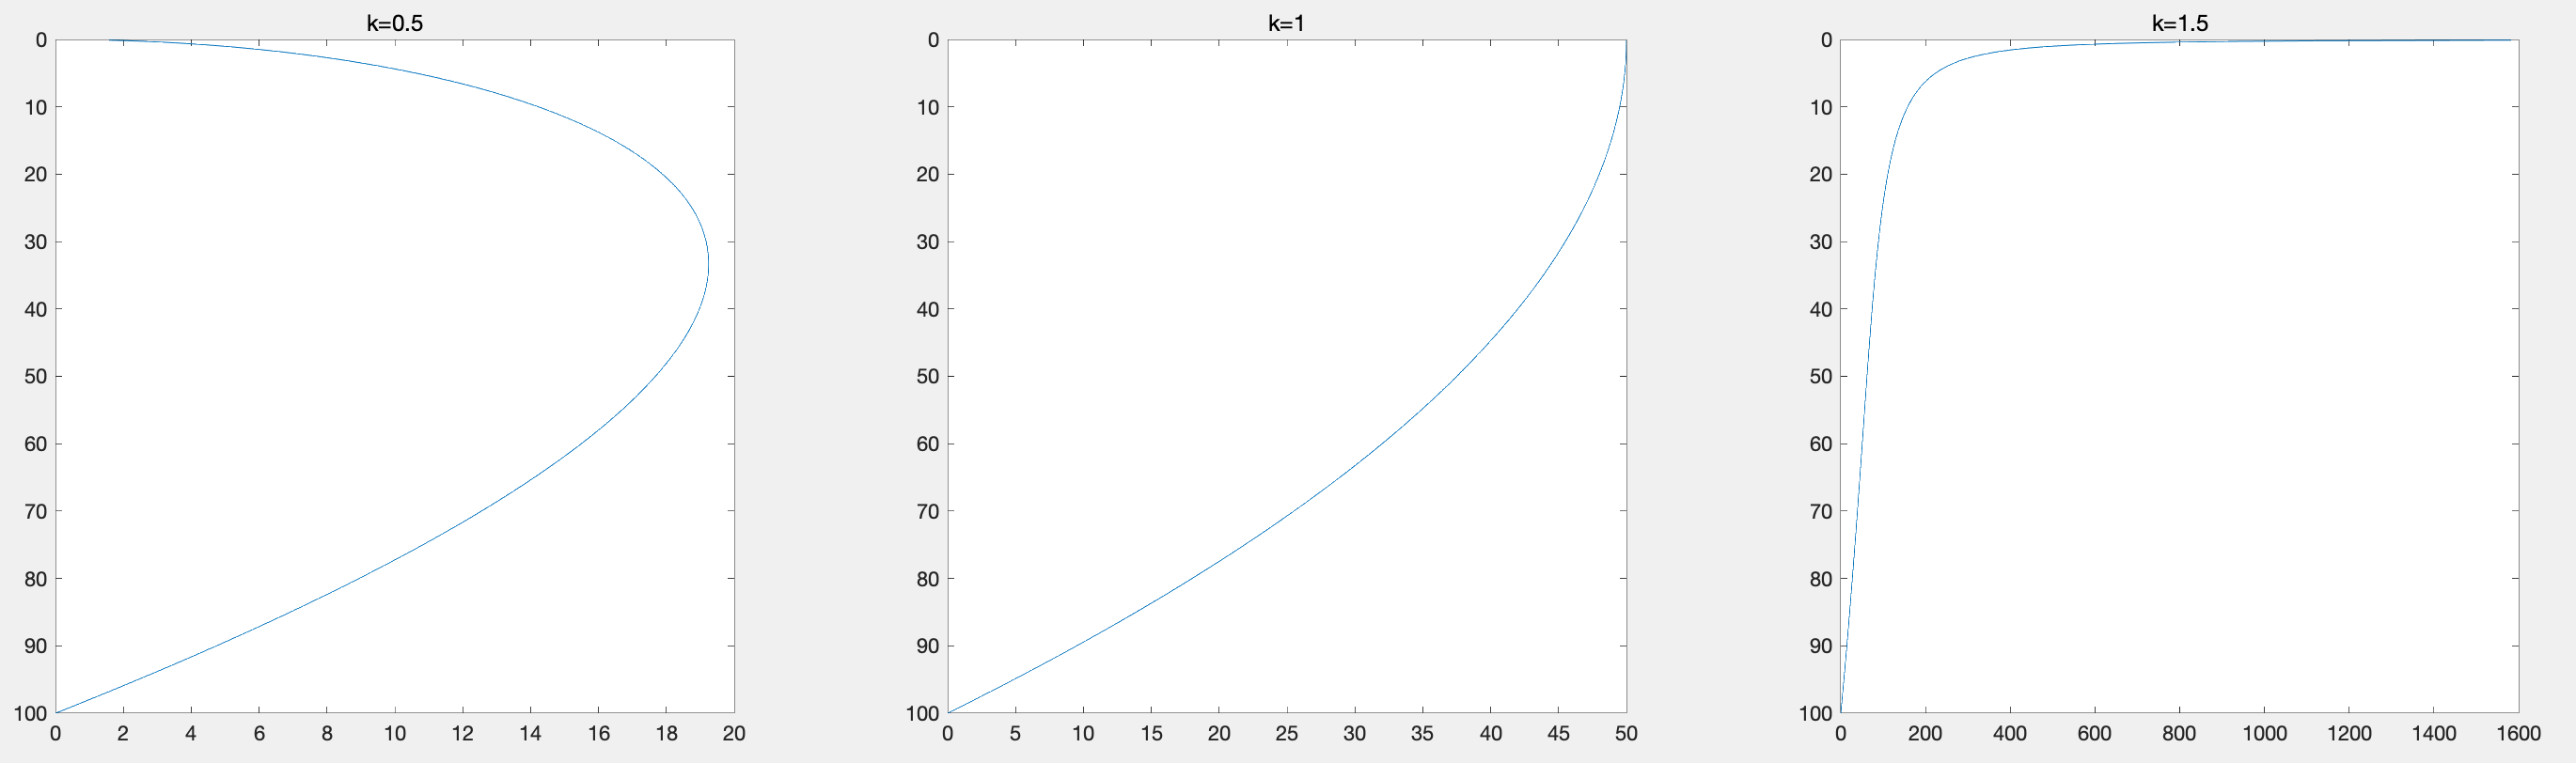
\includegraphics[width=1\textwidth]{pic1.png}
    \caption{不同k值下小船航行线路解析解图像}
\end{figure}


\subsection{设 d=100 m, v1 =1 m/s, v2 = 2 m/s。 用数值解法求渡河所需时间、任意时刻
小船的位置及航行曲线,作图,并与解析解比较;}

在小船航线和航行时间求解时,依然使用公式:
$$\frac{dx}{dt}=v_1-v_2cos\theta$$
$$\frac{dy}{dt}=-v_2sin\theta$$


且$sin\theta=\frac{y}{\sqrt{x^2+y^2}}$,$cos\theta=\frac{x}{\sqrt{x^2+y^2}}$。

给定时间精度之后,即可使用 MATLAB 中自带的 ode45函数进行求解任意时刻的小船 位置,将这些时刻的小船位置进行连接即可得到小船的航行曲线。当小船位置 y = 0 时,即 认为小船已经到达岸边,迭代结束。

MATLAB代码如下:

\begin{lstlisting}
%% Global Variables
global v1;
global v2;
v1 = 1;
v2 = 2;
k = v1 / v2;
d = 100;

%% Analyical Method
x_ana = 0:0.1:d;
y_ana = (x_ana ./ 2) .* ((d ./ x_ana) .^ k- (x_ana ./ d) .^ k);

%% Runge Kutta Method
ts = 0:1:100;
[t, xy] = ode45(@xypartial, ts, [0, d]);
x = xy(:,1);
y = xy(:,2);
% Trim x,y for better plot
x = max(x, 0);
y = max(y, 0);

figure;
set (gcf,'Position',[100,100,760,320])
subplot(1,2,1);
[AX] = plotyy(t,x,t,y);
grid on;
xlabel('Time');
legend('x(t)', 'y(t)');
subplot(1,2,2);
hold on;
plot(x, y);
plot(y_ana, x_ana, 'b--', 'LineWidth', 2); xlabel('x');
ylabel('y');
set(gca,'ydir','reverse')
legend('y(x)数值解', 'y(x)解析解');

%% Function
function [ dx ] = xypartial( t, x )
global v1;
global v2;
norm = sqrt(x(1) ^ 2 + x(2) ^ 2);
dx = [v1 - v2 * x(1) / norm; - v2 * x(2) / norm];
end
\end{lstlisting}


\begin{figure}[H]
    \centering
    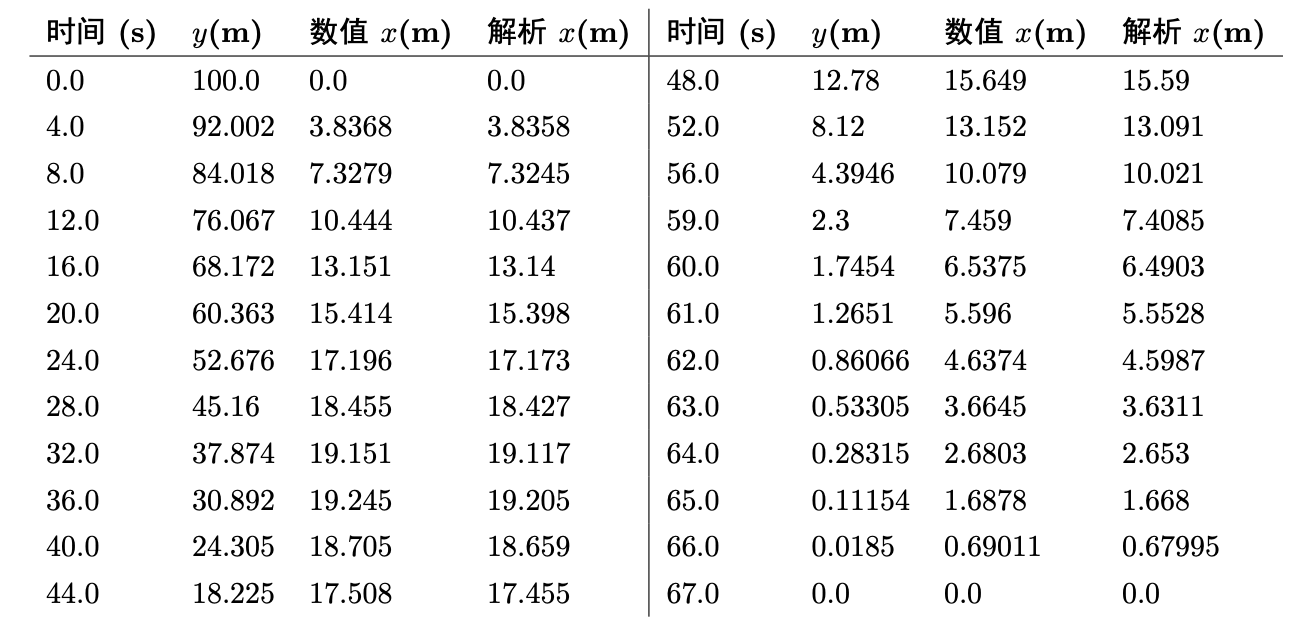
\includegraphics[width=0.7\textwidth]{table1.png}
    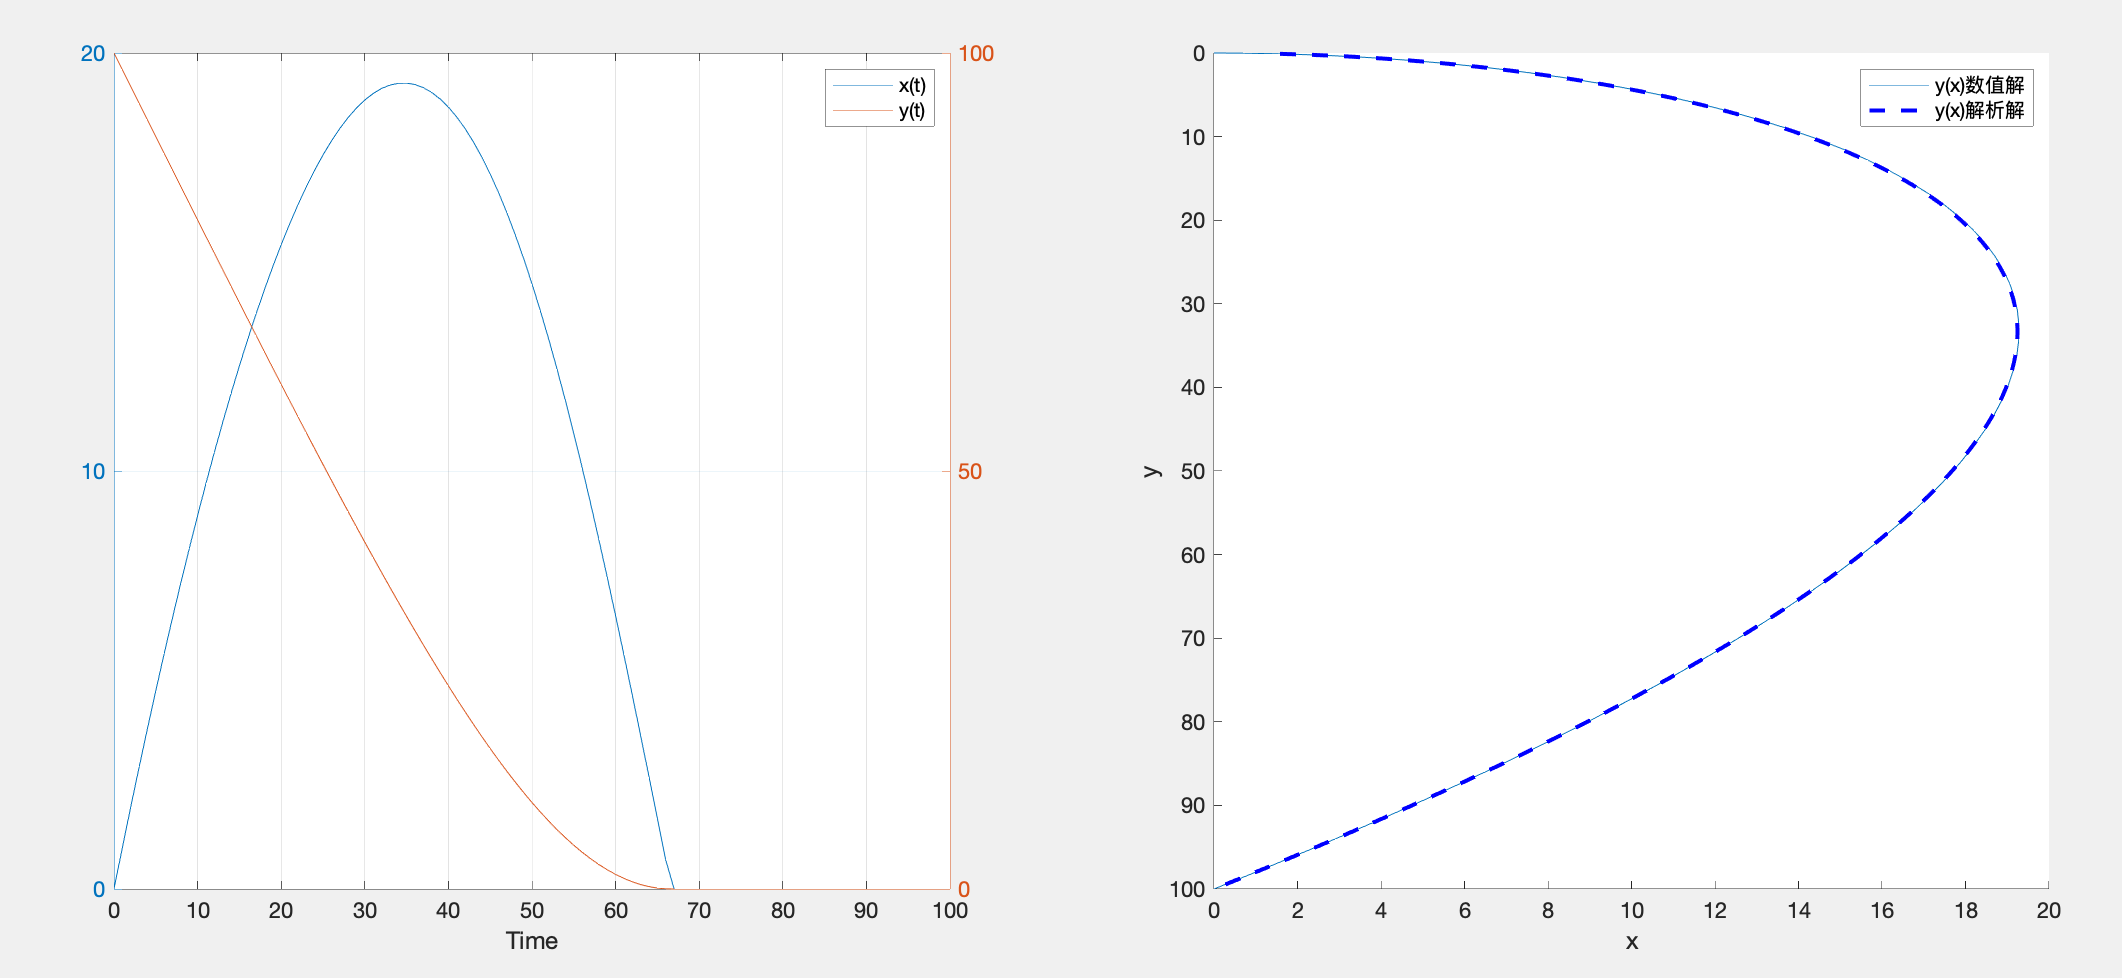
\includegraphics[width=0.7\textwidth]{pic2.png}
    \caption{$v_1=1.0m/s$时小船航行线路数据}
\end{figure}



从图表中可以清晰看出,数值解和解析解的结果比较相近,最终求得小船渡河所需的时间为 67 秒。


\subsection{若流速为 0, 0.5, 1.5, 2 (m/s),结果将如何。}
\begin{itemize}
\item{\textbf{$v_1=0.0m/s$}此时静水速度为0,小船理论上应该径直前进,最终求得小船渡河所需的时间为 50 秒。}
\item{\textbf{$v_1=0.5m/s$}数值解和解析解的结果由于累计误差稍有差别但大体相近,最终求得小船渡河所需的时间为 53.5 秒。}

\item{\textbf{$v_1=1.5m/s$}数值解和解析解的结果比较相近,最终求得小船渡河所需的时间为 114 秒。}
\item{\textbf{$v_1=2.0m/s$}极限情况下小船会在离终点 50m 处的位置附近,这与解析解的分析是一致 的。但是在数值求解的过程中,虽然 t 增大,但是小船始终与岸边有微小的距离,可以这样 分析:小船越靠近岸边,径向速度越慢,以至于最后所有的速度分量全部用于平衡水流速度。 但无论如何,小船在这种情况下始终无法到达 B 点。
}
\end{itemize}

\begin{figure}[H]
    \centering
    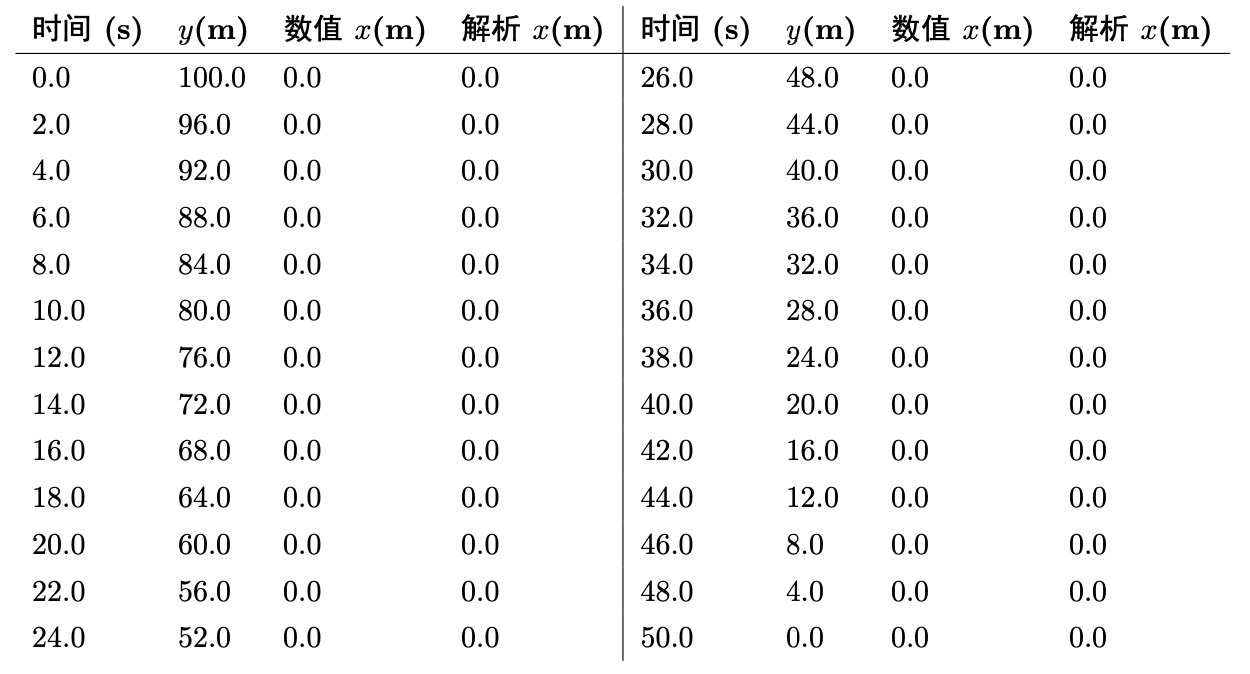
\includegraphics[width=0.7\textwidth]{v0.png}
    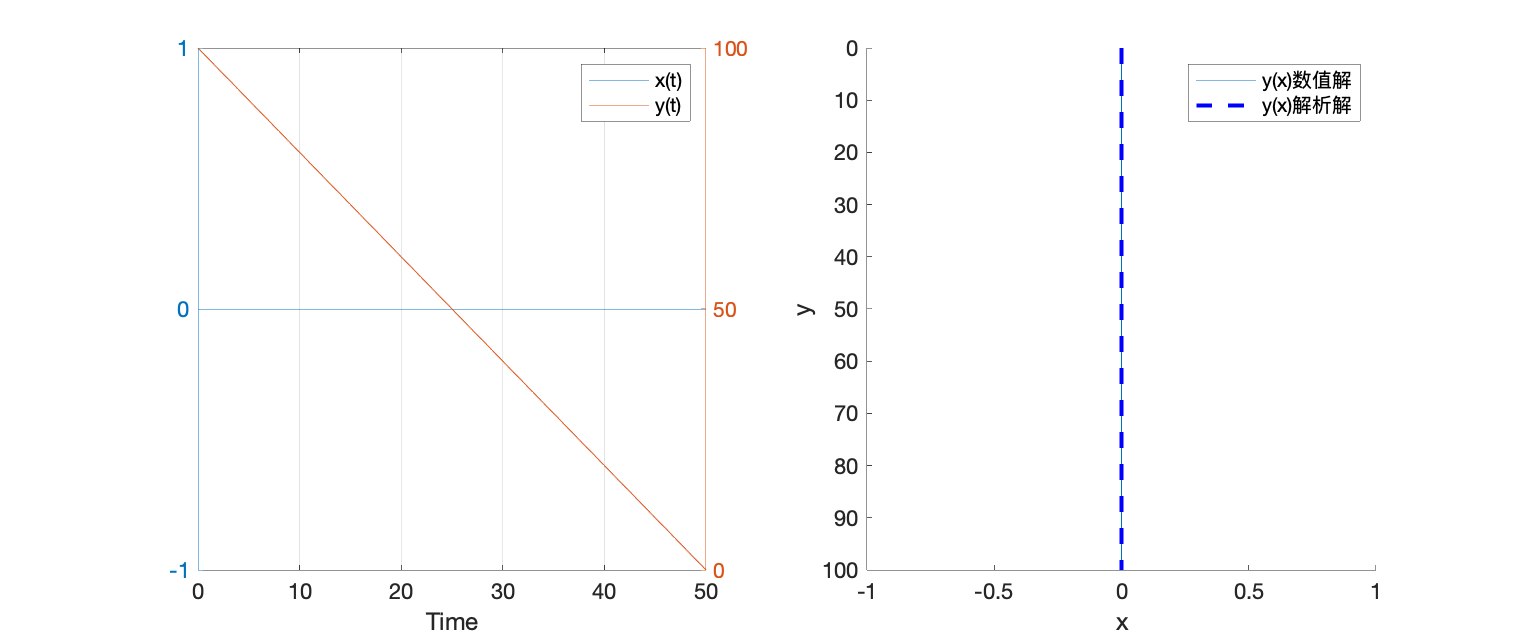
\includegraphics[width=0.7\textwidth]{pic3.png}
    \caption{$v_1=0.0m/s$时小船航行线路数据}
\end{figure}

\begin{figure}[H]
    \centering
    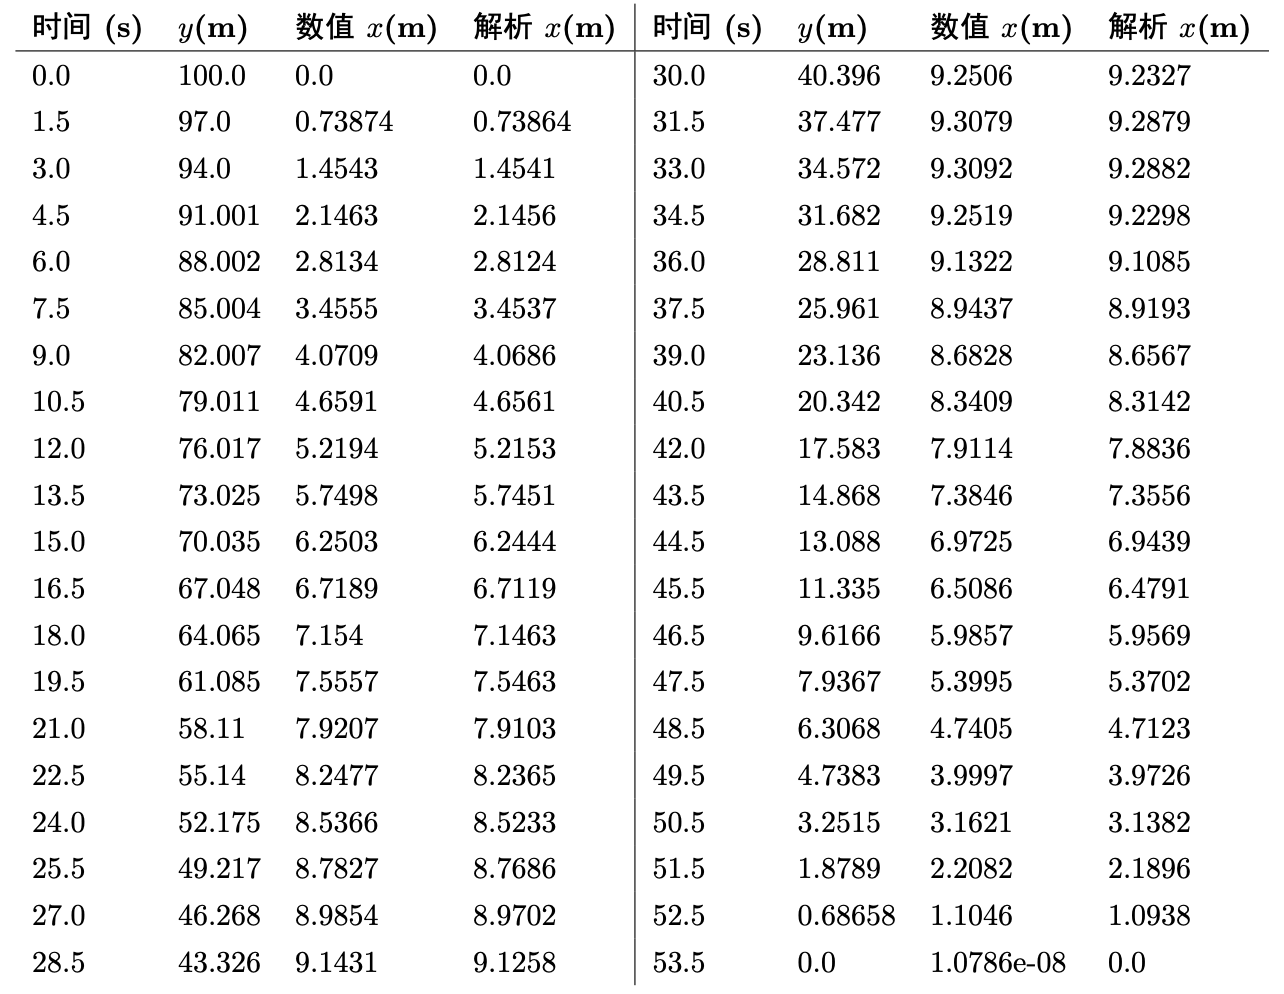
\includegraphics[width=0.7\textwidth]{v05.png}
    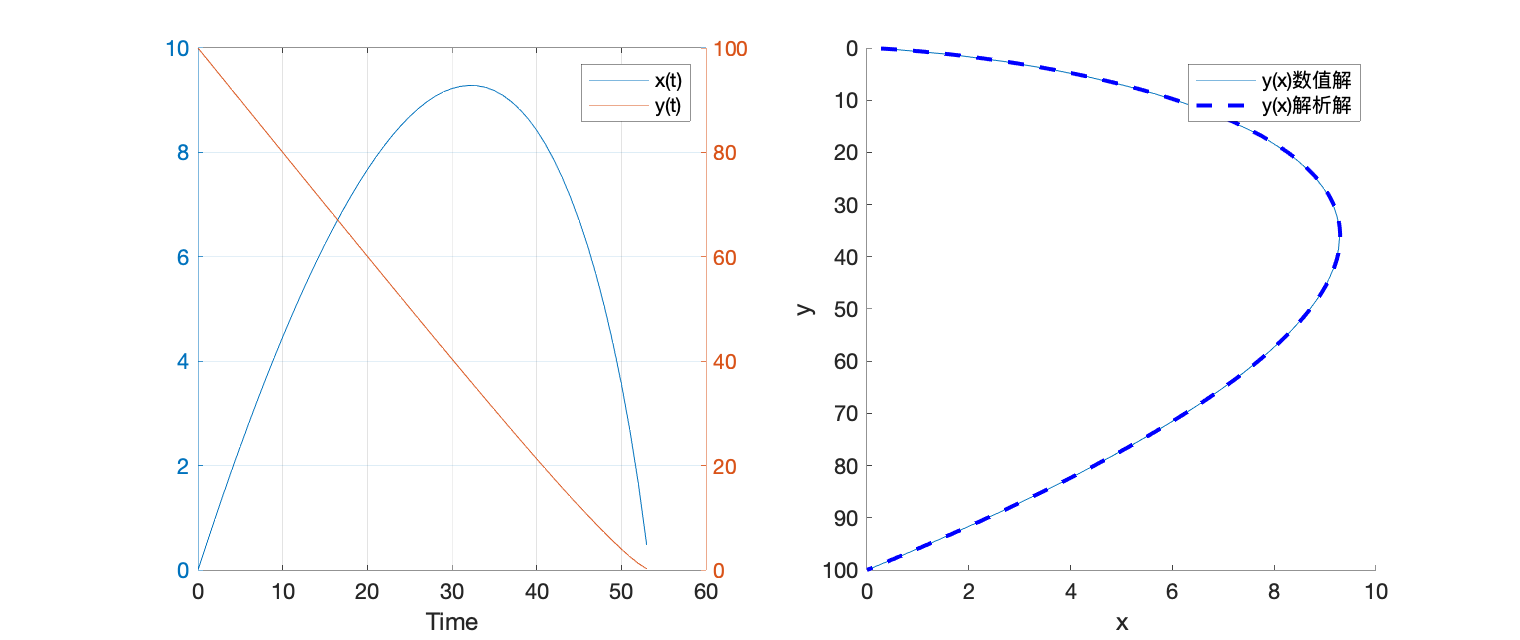
\includegraphics[width=0.7\textwidth]{pic4.png}
    \caption{$v_1=0.5m/s$时小船航行线路数据}
\end{figure}

\begin{figure}[H]
    \centering
    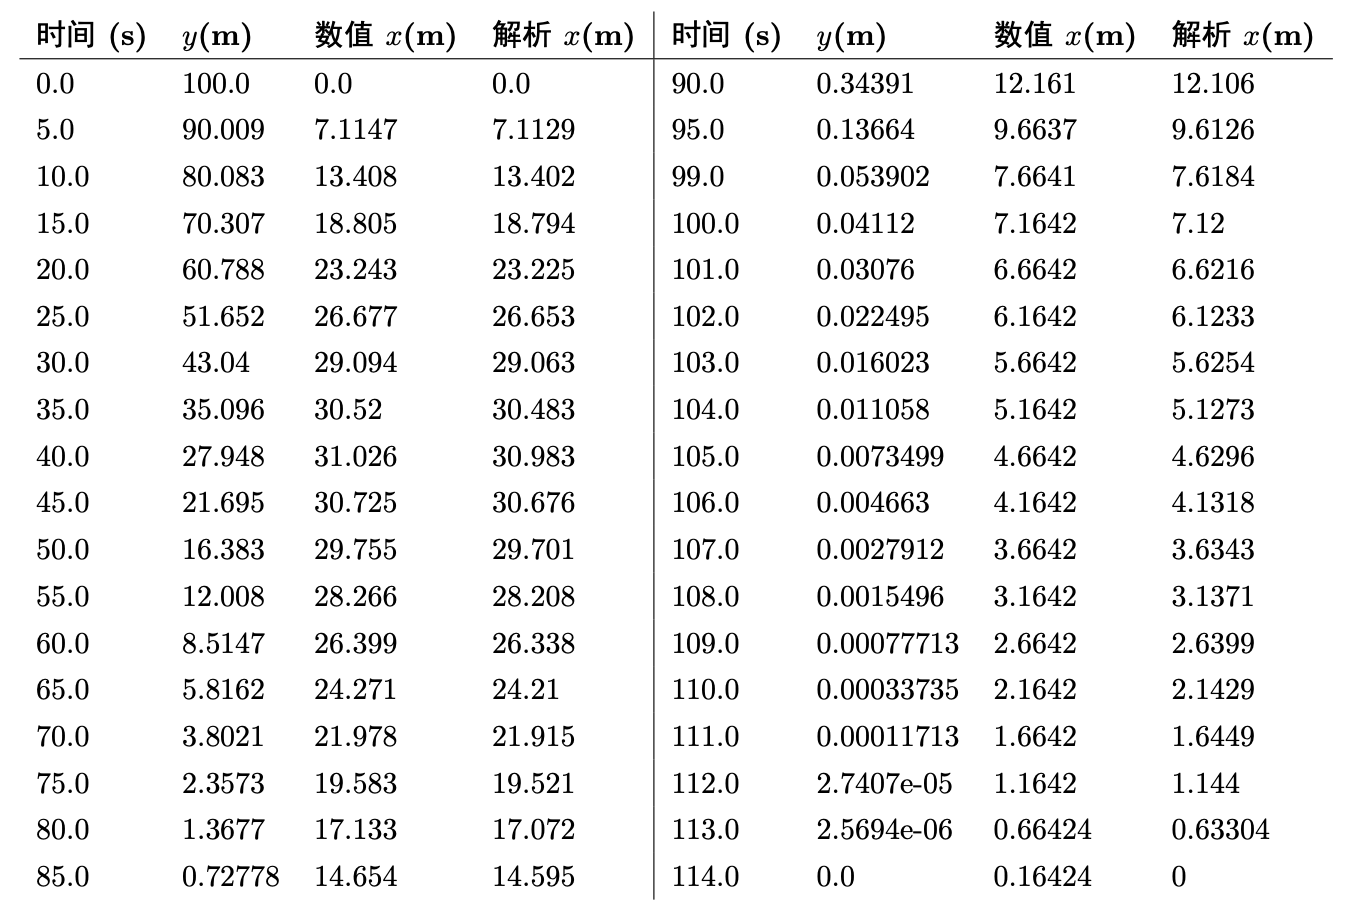
\includegraphics[width=0.7\textwidth]{v15.png}
    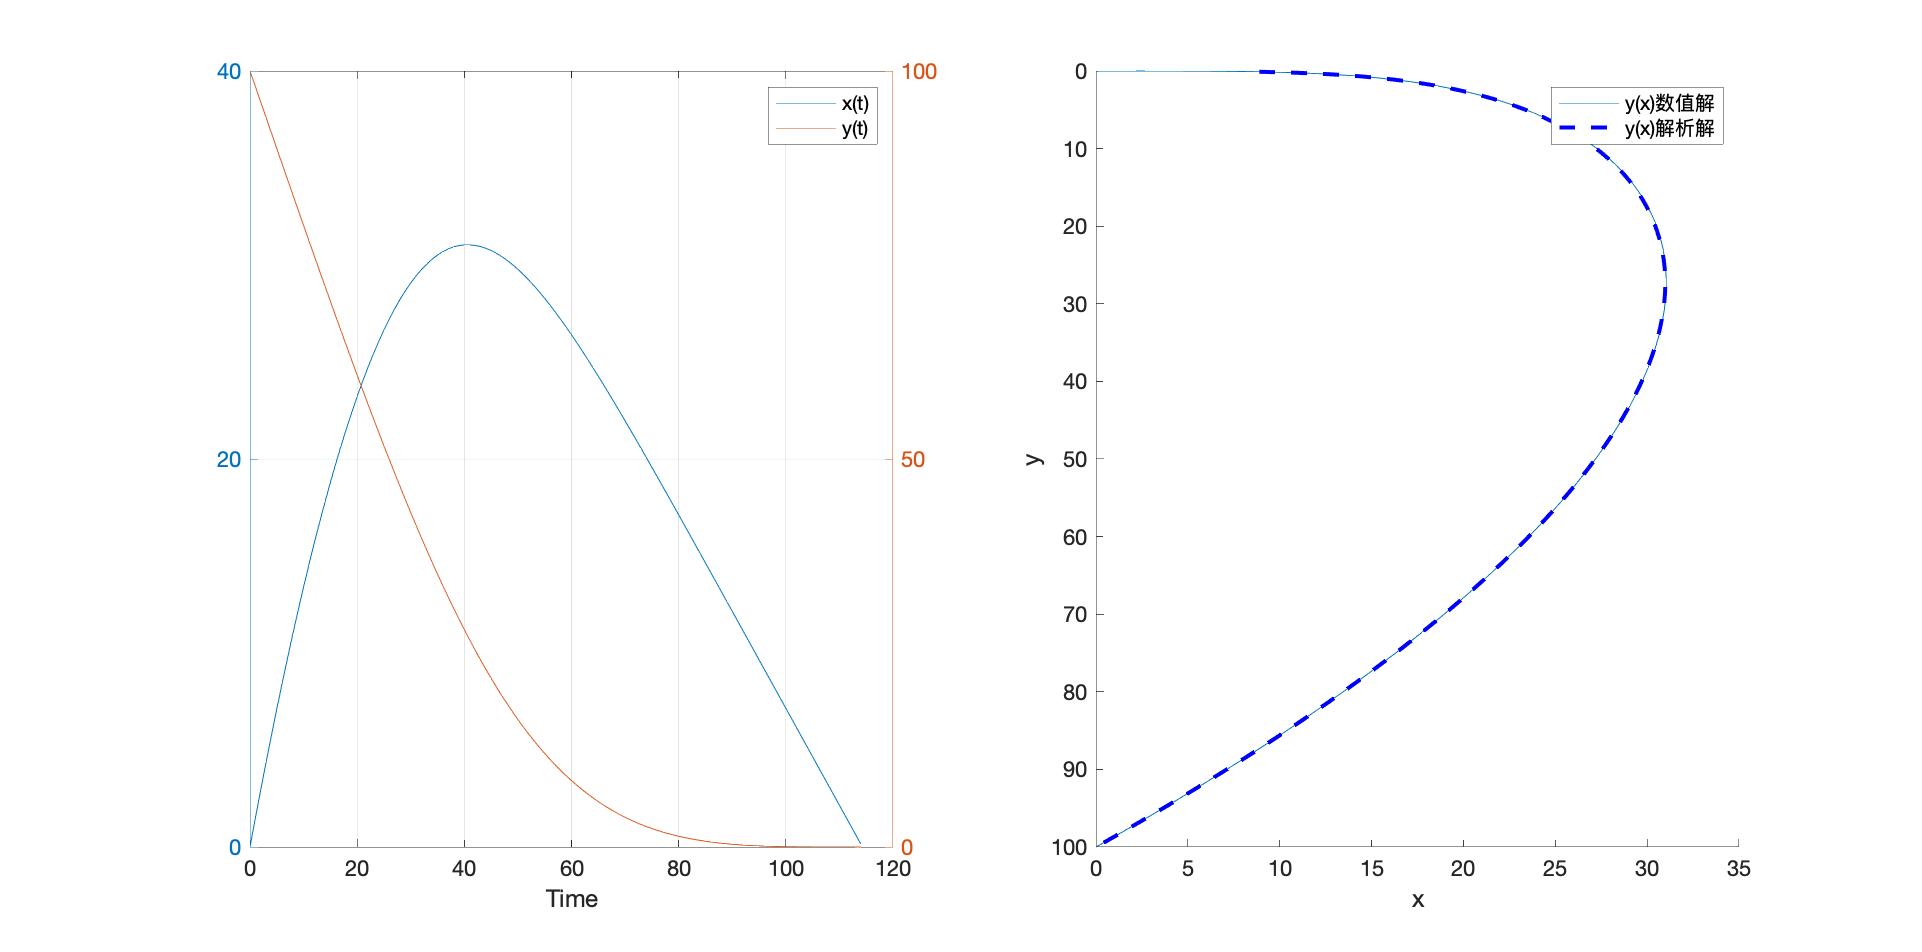
\includegraphics[width=0.7\textwidth]{pic5.png}
    \caption{$v_1=1.5m/s$时小船航行线路数据}
\end{figure}

\begin{figure}[H]
    \centering
    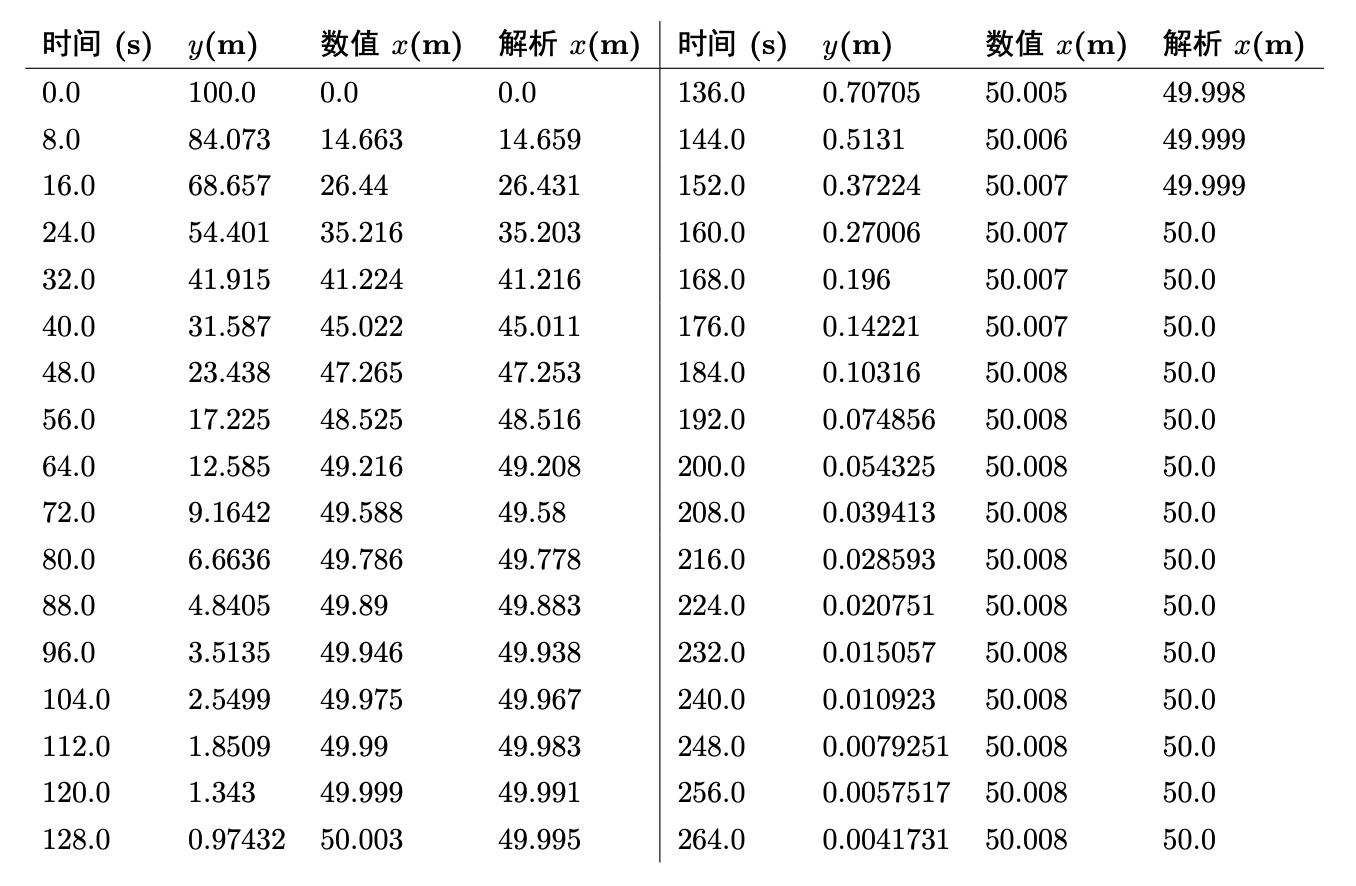
\includegraphics[width=0.7\textwidth]{v20.png}
    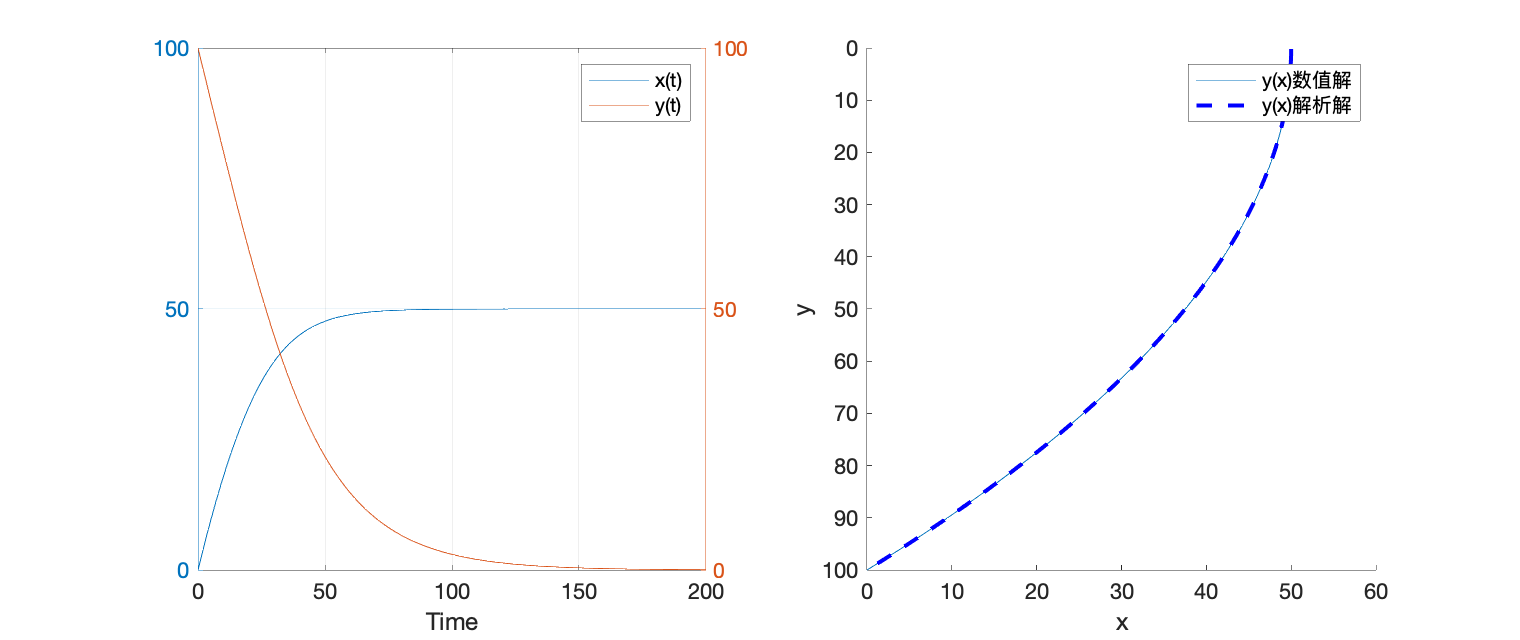
\includegraphics[width=0.7\textwidth]{pic6.png}
    \caption{$v_1=2.0m/s$时小船航行线路数据}
\end{figure}

\newpage

\section{CH4-T9 种群竞争}
\subsection{模型建立}
题目中已经建立模型。

\subsection{算法设计与代码实现}
ODE已由题目中给出,使用5级4阶龙格—库塔公式计算,并控制相对误差1e-6,绝对误差1e-9。
MATLAB代码如下:
\begin{lstlisting}
%% Gloabal Variables
%% Gloabal Variables
global r1;
global r2;
global n1;
global n2;
global s1;
global s2;
r1 = 1;
r2 = 1;
n1 = 100;
n2 = 100;
s1 = 0.5;
s2 = 2;

%% Solve
ts=[0:0.1:30];%时间区间
x0=[10,10];%初始条件
opt=odeset('reltol',1e-6,'abstol',1e-9);%相对误差1e-6,绝对误差1e-9
[t,x]=ode45(@odeFunc,ts,x0,opt);

figure;
grid on;

subplot(1,2,1);
hold on;
plot(t,x(:,1),'LineWidth',2);
gtext('x(t)');
plot(t,x(:,2),'LineWidth',2);
gtext('y(t)');
hold off;

subplot(1,2,2);
plot(x(:,1),x(:,2),'LineWidth',2);
xlabel('x');
ylabel('y');


%% Function
function dx = odeFunc(t, x)
global r1;
global r2;
global n1;
global n2;
global s1;
global s2;
dx = [r1*x(1)*(1-x(1)/n1-s1*x(2)/n2); r2*x(2)*(1-s2*x(1)/n1-x(2)/n2)];
end
\end{lstlisting}

\subsection{(1)}
在 $r_1=r_2=1, n_1=n_2=100, s_1=0.5, s_2=2, x_0=y_0=10$的情况下,x(t)图形,y(t)图形及相图(x, y)如下图所示:
\begin{figure}[H]
    \centering
    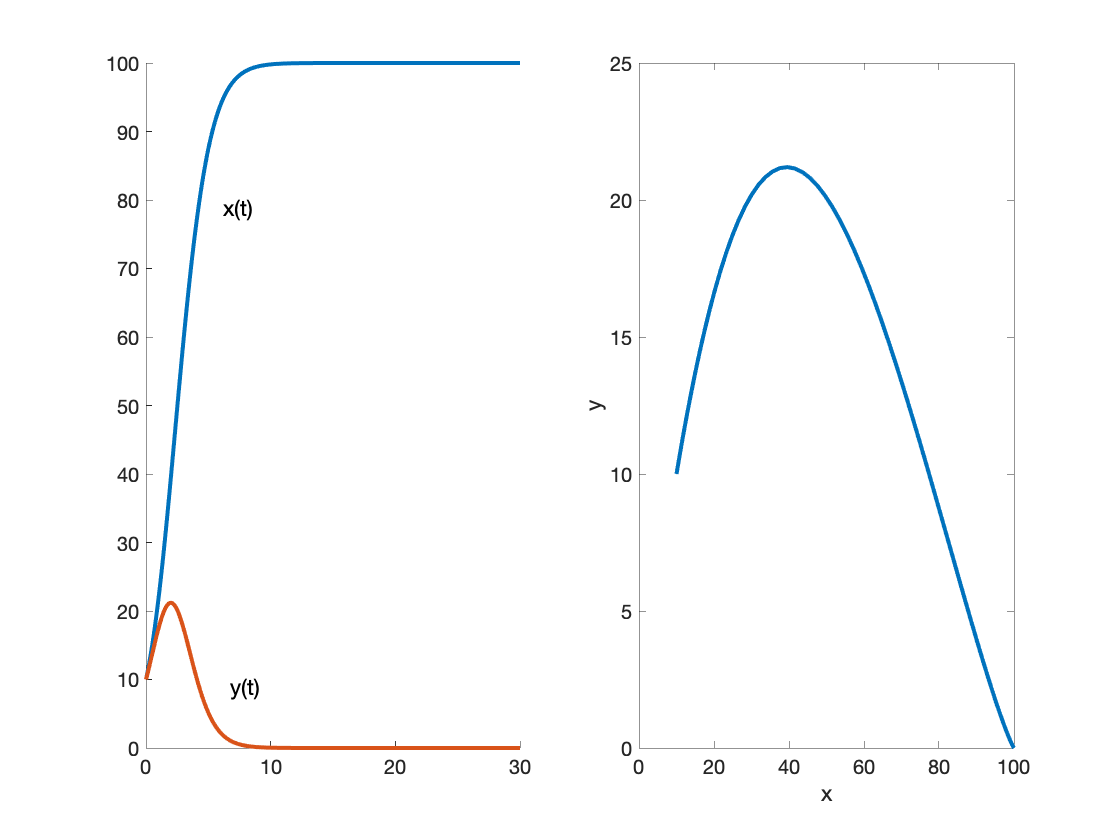
\includegraphics[width=0.7\textwidth]{pic91.png}
    \caption{$r_1=r_2=1, n_1=n_2=100, s_1=0.5, s_2=2, x_0=y_0=10$}
\end{figure}
图中可以看出最后数值稳定在x=100,y=0上,即物种甲达到最大值,物种乙灭绝。

\subsection{(2)}
以第一小题为基准,设置$r_1=r_2=0.3$得到如下图形:
\begin{figure}[H]
    \centering
    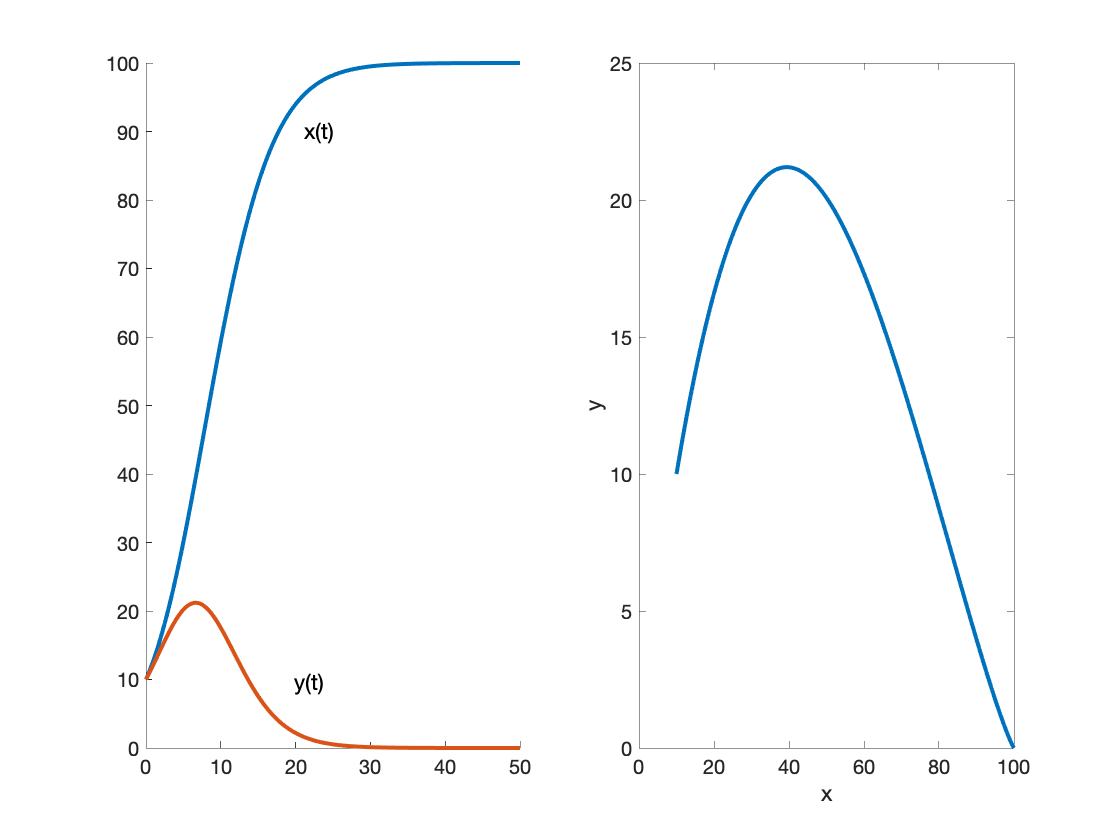
\includegraphics[width=0.7\textwidth]{pic92.png}
    \caption{$r_1=r_2=0.3, n_1=n_2=100, s_1=0.5, s_2=2, x_0=y_0=10$}
\end{figure}
我们可以看到甲乙两物种最终结果仍然是甲达到数量极限而乙灭绝,但与原先不同的是变化速度减缓了,这是由于自然增长率r1,r2变小的缘故(相当于变化率减小)。

以第一小题为基准,设置$n_1=10000,n_2=100$得到如下图形:
\begin{figure}[H]
    \centering
    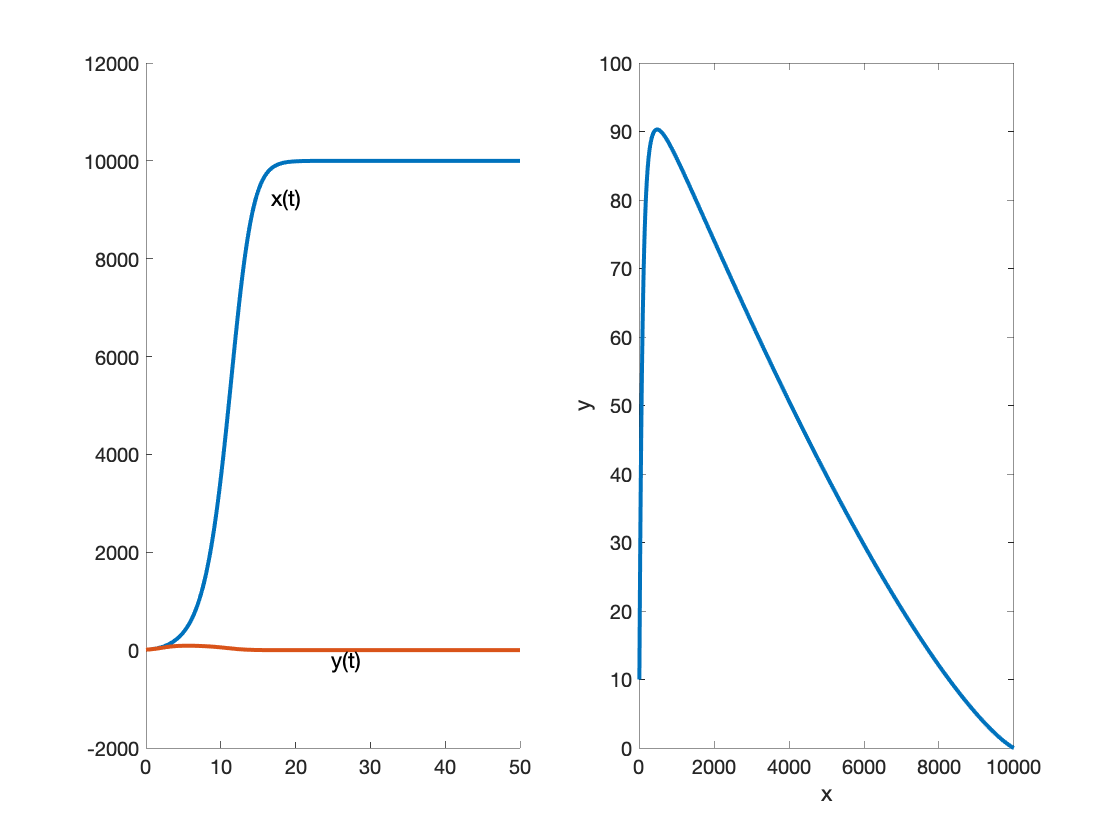
\includegraphics[width=0.7\textwidth]{pic93.png}
    \caption{$r_1=r_2=1, n_1=10000, n_2=100, s_1=0.5, s_2=2, x_0=y_0=10$}
\end{figure}
由于一开始甲物种的数量相对较少,所以乙物种得以快速增长,数量一度达到90以上,但最终仍然灭绝。物种容量的改变并不能影响最终谁会灭绝.

以第一小题为基准,设置$x_0=10,y_0=100$得到如下图形:
\begin{figure}[H]
    \centering
    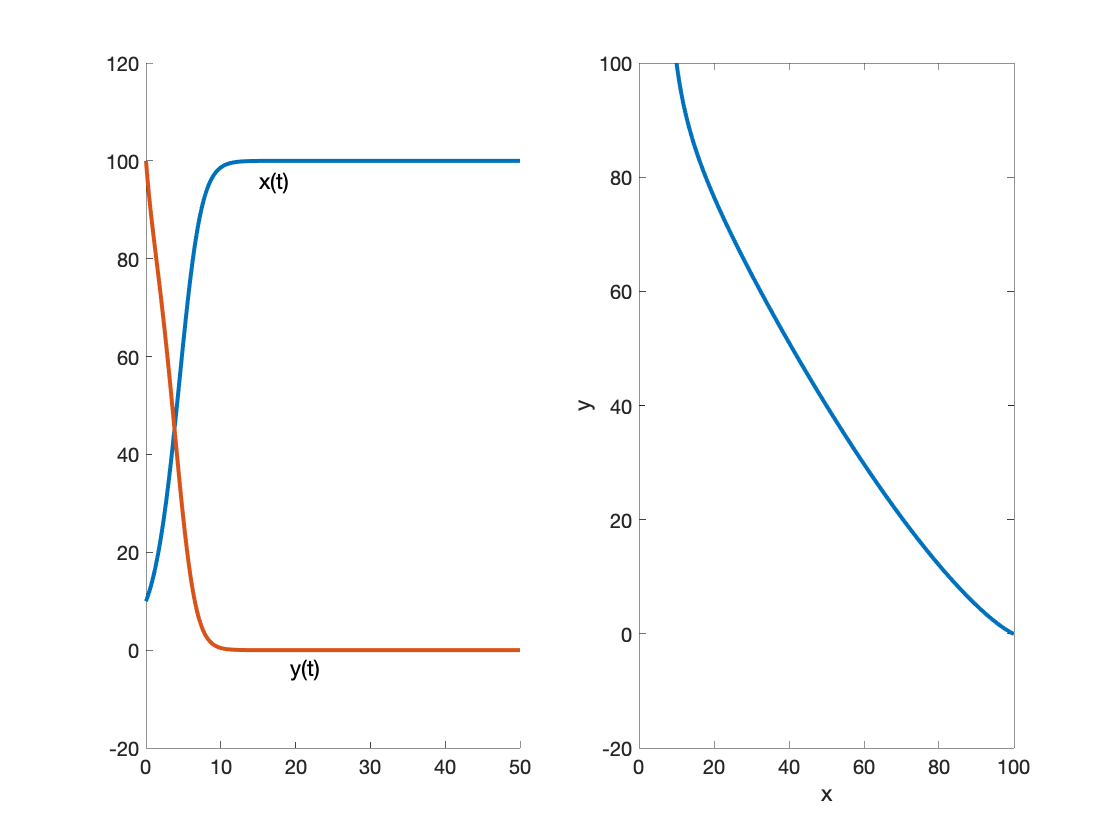
\includegraphics[width=0.7\textwidth]{pic94.png}
    \caption{$r_1=r_2=1, n_1=n_2=100, s_1=0.5, s_2=2, x_0=10, y_0=100$}
\end{figure}
乙物种的初始数量大使其灭绝时间稍稍延后,但它灭绝的趋势不变。

\textbf{综上,无论怎样改变$r_1,r_2,n_1,n_2,x_0,y_0$,都改变不了最后甲物种存活并达到数量最大且乙物种灭绝的结果。}

以第一小题为基准,设置$s_1=1.5,s_2=0.7$得到如下图形:
\begin{figure}[H]
    \centering
    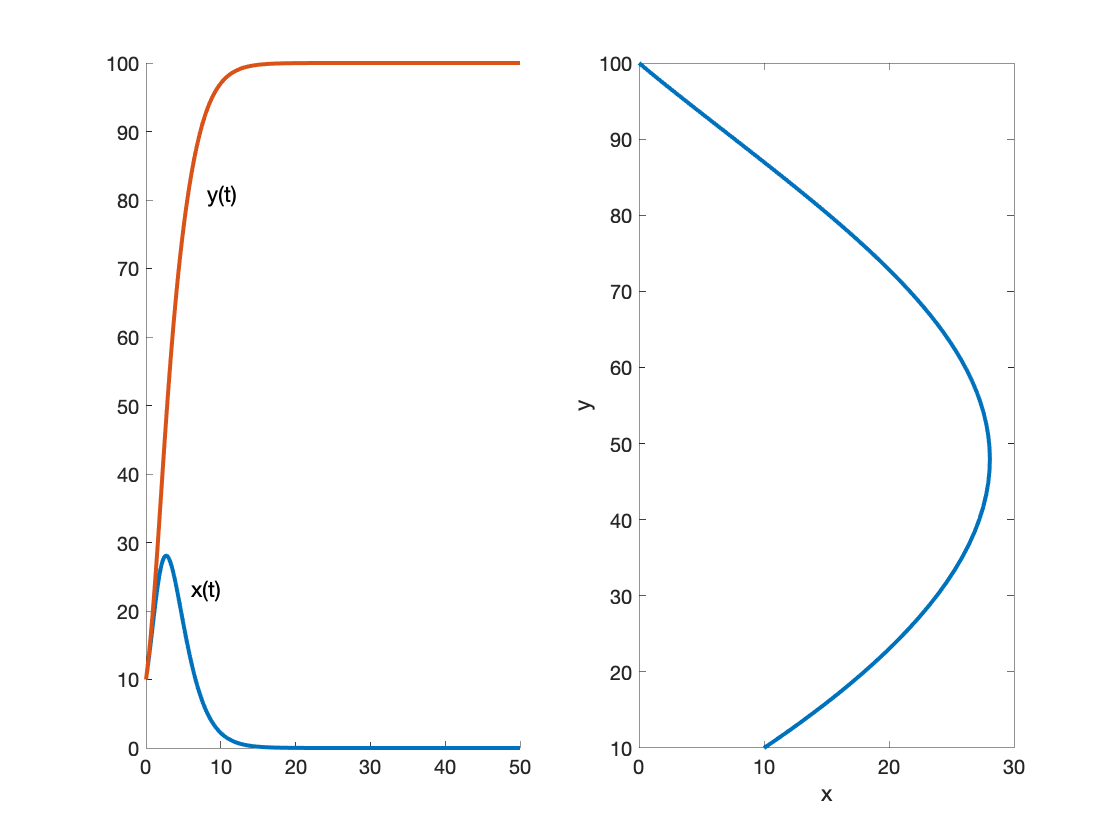
\includegraphics[width=0.7\textwidth]{pic95.png}
    \caption{$r_1=r_2=1, n_1=n_2=100, s_1=1.5, s_2=0.7, x_0=y_0=10$}
\end{figure}
最后甲物种灭绝,乙物种存活并达到数量极限。

所以$s_1,s_2$对两物种在自然界长期演变的结局起决定作用。下面在第三小题中进一步讨论$s_1,s_2$对物种的影响。

\subsection{(3)}
设置$s_1=0.8(<1),s_2=0.7(<1)$得到如下图形:
\begin{figure}[H]
    \centering
    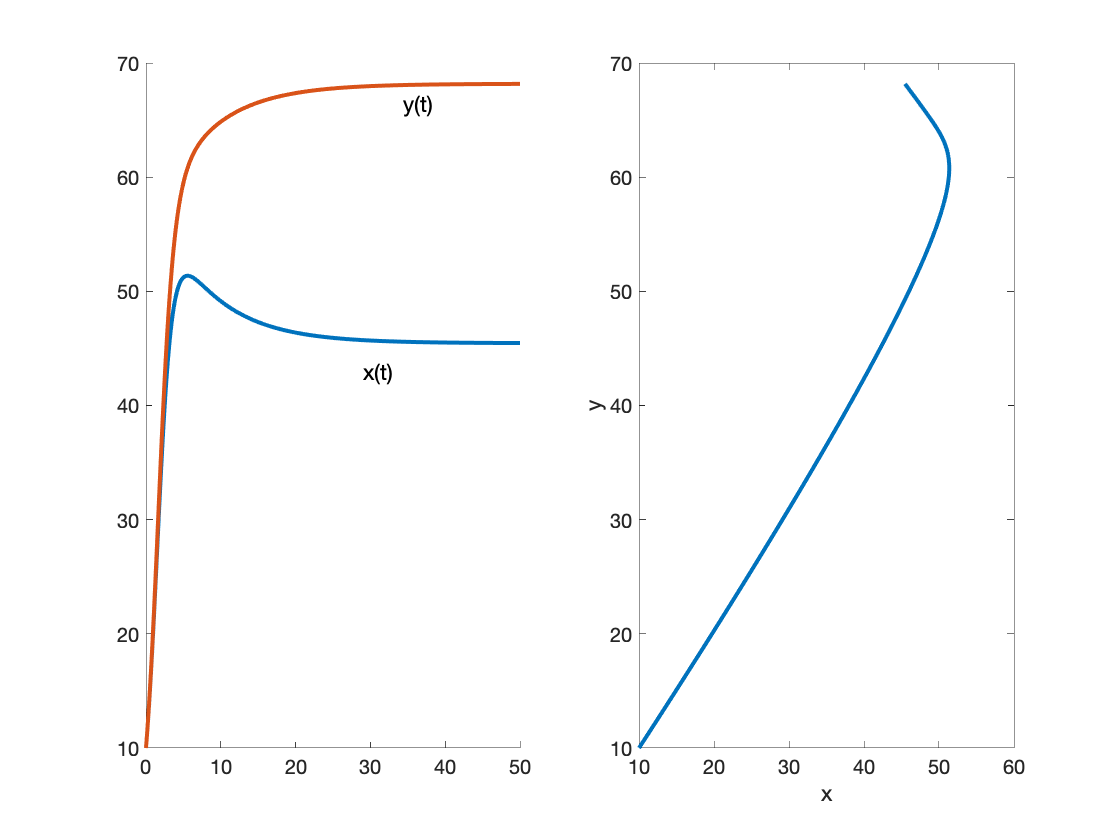
\includegraphics[width=0.7\textwidth]{pic96.png}
    \caption{$r_1=r_2=1, n_1=n_2=100, s_1=0.8, s_2=0.7, x_0=y_0=10$}
\end{figure}
最后稳定在了$x=45,y=68$。

设置$s_1=1.5(>1),s_2=1.7(>1)$得到如下图形:
\begin{figure}[H]
    \centering
    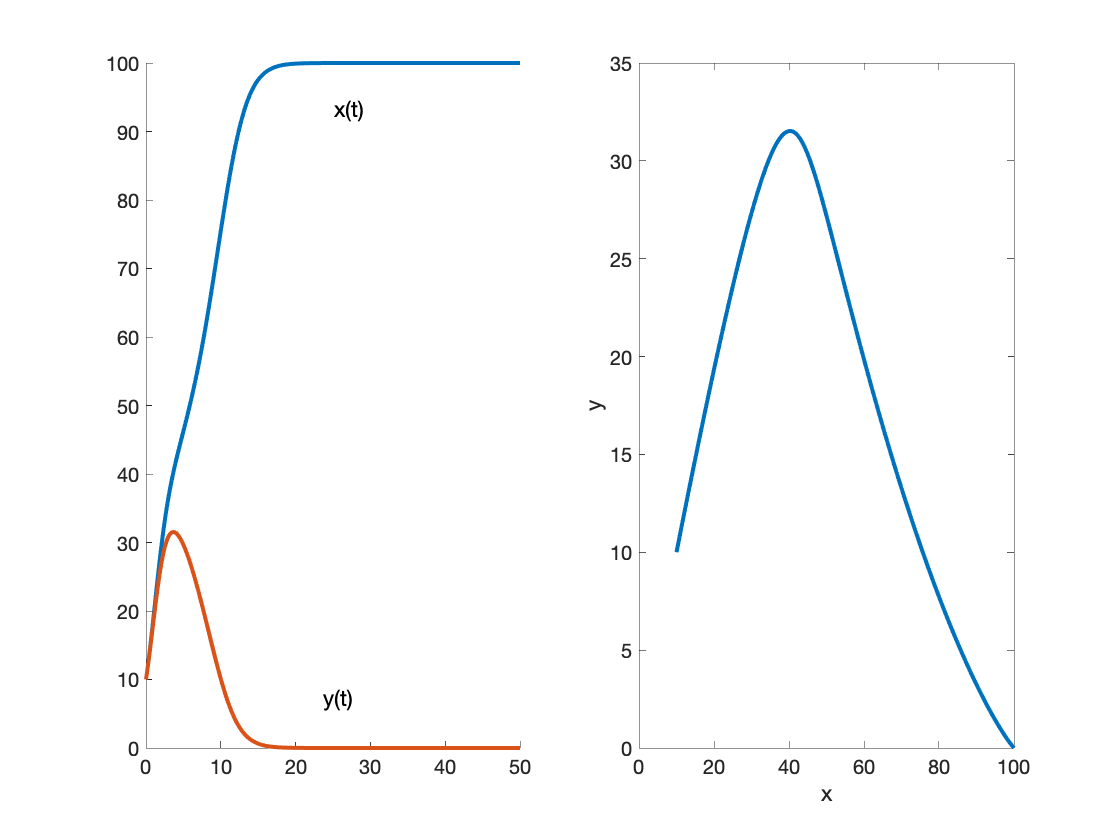
\includegraphics[width=0.7\textwidth]{pic97.png}
    \caption{$r_1=r_2=1, n_1=n_2=100, s_1=1.5, s_2=1.7, x_0=y_0=10$}
\end{figure}
虽然$s_1,s_2$都大于1,但是$s_2$更大,严重消耗了乙物种的生存资源,使乙物种在竞争中灭绝。

设置$s_1=s_2=1.6(>1)$得到如下图形:
\begin{figure}[H]
    \centering
    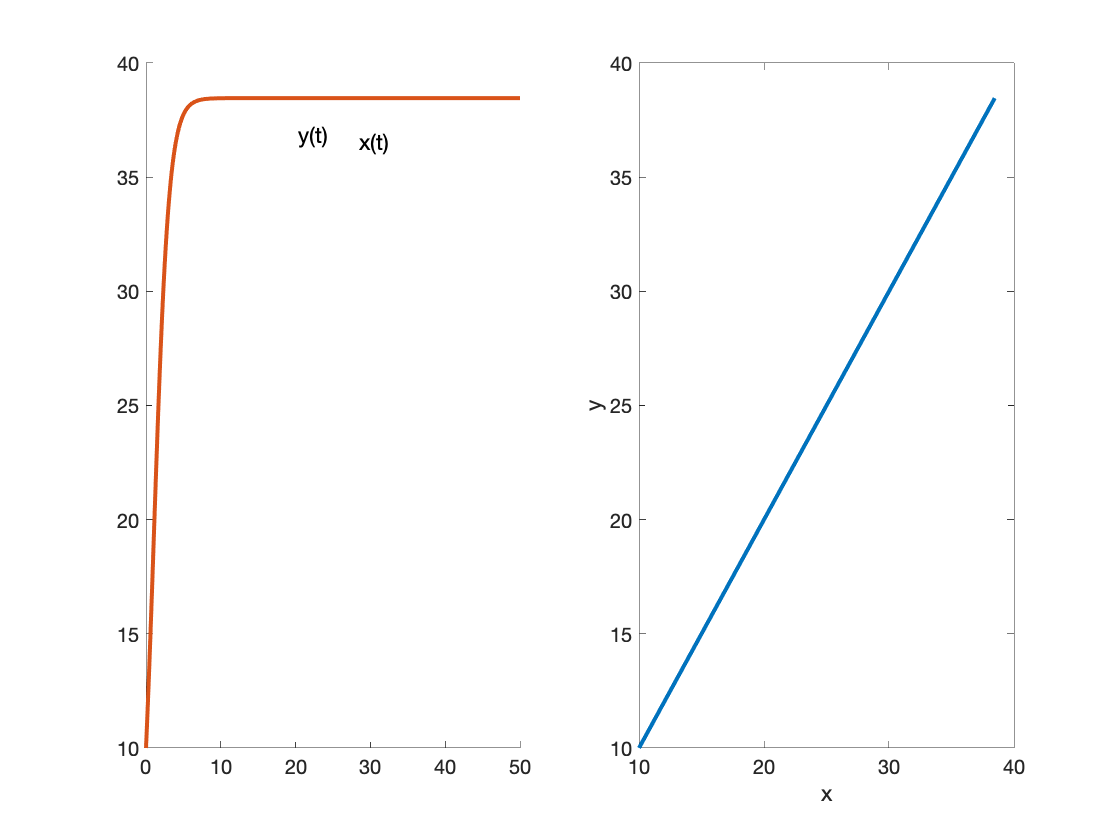
\includegraphics[width=0.7\textwidth]{pic98.png}
    \caption{$r_1=r_2=1, n_1=n_2=100, s_1=s_2=1.6, x_0=y_0=10$}
\end{figure}

设置$s_1=s_2=0.6(<1)$得到如下图形:
\begin{figure}[H]
    \centering
    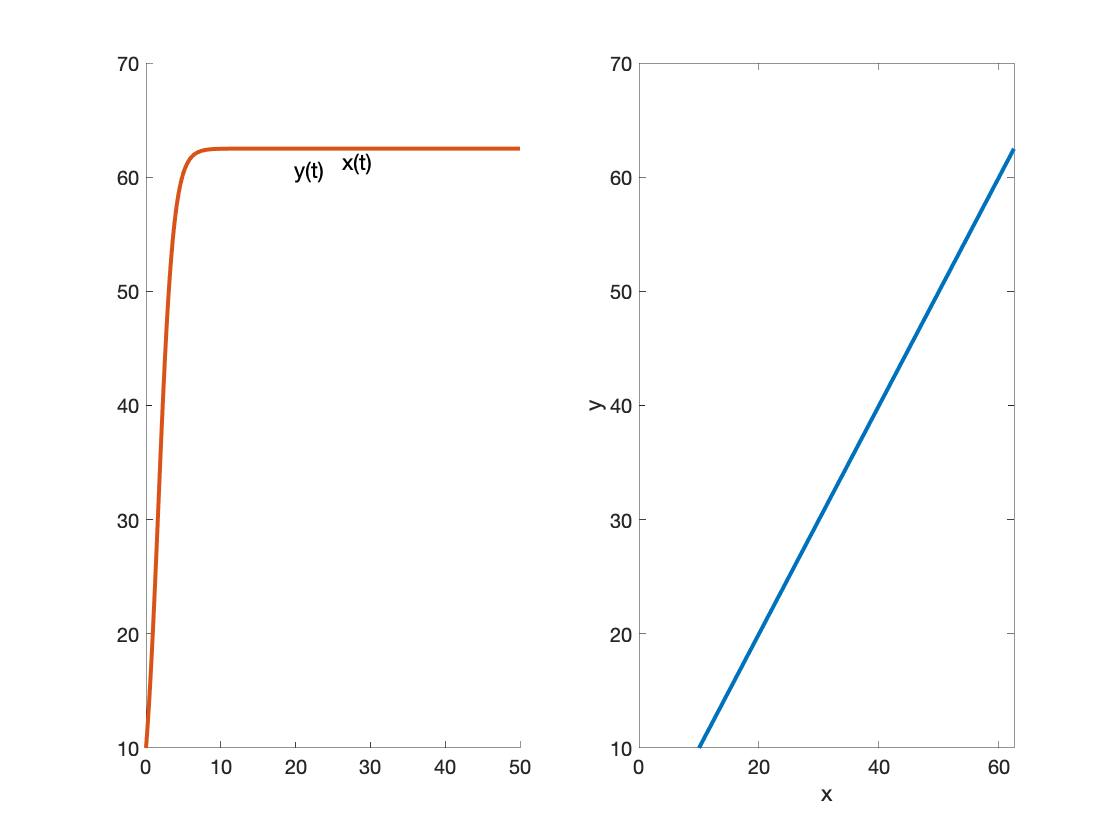
\includegraphics[width=0.7\textwidth]{pic99.png}
    \caption{$r_1=r_2=1, n_1=n_2=100, s_1=s_2=0.6, x_0=y_0=10$}
\end{figure}
当$s_1,s_2$相等的时候,两者可以共生。当$s_1,s_2>1$时,代表两物种消耗资源比较大,最终稳定的物种数量要小于$s_1,s_2<1$的时候。

\textbf{结论}

当$s_1,s_2<1$时,消耗生存资源的严重程度较轻,所以甲乙物种可以共存,但两者都达不到最大值;

当$s_1,s_2>1$时,两物种竞争激烈,最后s1,s2中更大者对应作用的物种灭绝。所谓物尽天择,自然资源是有限的,需要更少资源就能生存的物种在竞争中将占有优势。

当其中之一大于1时,对应作用的物种就会由于生存资源的过度消耗而灭绝;

当$s_1=s_2$时,都大于1但相等时,由于方程的对称性,甲乙两物种都能生存下来,但都不能达到最大值。


\newpage
\section{收获和建议}
通过这次的实验,我对 MATLAB 中提供微分方程求解函数理解更加深刻,通过实际编 程、画图的方式观察了方程求解的结果,这是书本上无法学到的知识。同时,在做上机实验 的过程中,我对 MATLAB 这款软件的使用也更加熟练了。希望在之后的课堂上老师能够当 堂进行相关的技巧演示并给出题目的分步解答。

\end{document}